%!TEX root = ../Thesis.tex
\chapter{Selection permeation enhancers}

In agreement with Novo Nordisk. The specific methods of combining permeability predictions and solubility predictions and the actual suggested candidates have not been included in this thesis. However the distribution of solubility predictions and permeation predictions is a good basis for a discussion of whether it is possible to find permeation enhancers that are both soluble and sufficiently potent.


\subsection{Is predicted potency the same as insolubility}
In Figure \ref{predictionsCombined} the predicted solubility and permeability is plotted for 10,000 molecules. Permeability predictions is based on a model similar to the one described in article of Section \ref{article:predAbs}. As the predictive model rely molecular descriptor computations with the MOE software suite, and these take in average 1 second per molecule. The full available million molecule search set would have taken 11 days to run. To narrow down the search set, molecules were selected by criteria of rotatable bonds and molar weight, in anticipation that molecules with less than a certain fraction of rotatable bonds likely would not have a fatty carbon chain, required to be an efficient surfactant-like permeation enhancer.

As discussed in Section \ref{predPerm:workflow} a major consideration was that the permeability model and solubility model both only would recognize lipophilicity-like properties as predictors, and thus perform exactly opposite predictions. However this seems not to be the case for the 10,000 predicted molecules. 

\begin{figure}[!htbp]
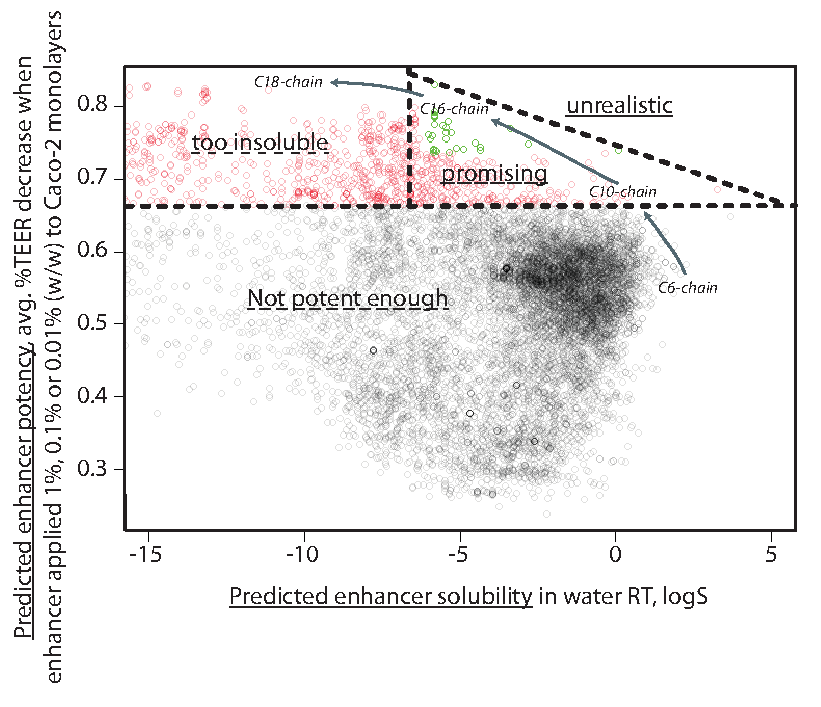
\includegraphics[width=\textwidth,height=\textheight,keepaspectratio]{graphics/screened_molecules3.pdf}
\caption{Predictions of logS water solubility and permeation enhancement in Caco-2 model for 10,000 compounds. Few molecules are both soluble and potent permeation enhancers. Figure have been segmented into groups of 'too insoluble', 'not potent enough', 'promising' and 'unrealistic'. For group of surfactant permeation enhancer the carbon chain can reduced or elongated. C6 to C18 exemplify a given enhancer group, where the C18 is too insolble and C6 not potent enough. A given other enhancer family with less favorable head group may never cross into the 'promising' segment for any carbon chain length.}
\label{predictionsCombined}
\end{figure}

In Figure \ref{predictionsCombined} the majority of molecules are not potent enough. Sodium caprate has been set as the lower bar of required potency = 0.67. A potency of 0.67 predicts that if a compound was used as permation enhancer and added to three Caco-2 monolayers in solution at 1\%, 0.1\% and 0.01\% \textit{(w/w)}, the lower electrical resistance across the three monolayers would in average be lowered 67\%. As dicussed in article from Section \ref{article:predAbs}, the permeation model overestimate the potency of non permeation enhancers, as the training set contained non permation enhancers. Thus the model likely cannot separate non potent from weekly potent. However, a permeation enhancement potency below C10 is probably too weak. As no C8 or C6 permation enhancers have been succesfully included in a formulation.

\subsection{Uncertainty of predictions}
In Section \ref{article:predAbs} the root mean square prediction error of the permeation enhancer model was found to 0.16, on the defined potency scale from 0 to 1. The prediction error was estimated by cross-validation and on a external data set. Therefore it is reasonable to expect the model can recognize molecules as highly potent, medium potent or non-potent permeation enhancers. The prediction error (stand deviation) of the solubility model as discussed in the results part of the draft "Learning the structure of random forest models QSAR modelling: Predicting molecular Solubilty" in Section \ref{article:solubility} estimated by cross-validation is 0.64 on the logS scale. A standard deviation on logS scale translates to a 4-fold deviation. As the training molecules in the Huskonnen data set \cite{palmer2007random} span the logS scale from -10 to +2, a a prediction error of 0.64(RMSE) seems as a quite accurate model. Likewise, the cross-validated estimated explained variance of the model is 90\%. However to function as an permeation enhancer, if logS is below -6, the dissolution rate will likely be too slow. Most surfactant based permeation enhancers have an ability to form micelles such that the an apparent solubility of very lipophilic permeation enhancers could be close -1 anyhow, as the solution is loaded with micelles. However the lipophilic permeation enhancer will have a low dissolution rate. The predictions of a theretical logS with micelles replaces the intrinsic dissolution rate, that likely would have been the property. No large public data sets was found for intrinsic dissolution. Therefore, although the solubility model seem to have a higher accuracy than the permeation model, the fact that only a narrow band of logS is useful and that logS is a substitution intrinsic dissolution rate.


\section{Discussion}

Permeation enhancers can increase the permeability of insulin across the epithelial barrier. Insulin degrade with time due to enzymes in the luminal space of the small intestine. To reduce the time in luminal space, the permeation enhancer must contribute to a fast efficient dissolution of the tablet. A very slow release will give zero-order enzyme reactions an advantage to break down all insulin. Also the permeation enhancer may cleared from the site of action faster than the release from the tablet, thus the overall concentration of permeation enhancer in the epithelial membrane will be to low

Identifying new potent enhancers with the Caco-2 cell model do not emphasize the dissolution speed. As a substitute for intrinsic dissolution speed measurements, logS-solubility was used instead, as intrinsic dissolution measurements were too sparse and not available in the public domain. Predicting both solubility and permeation enhancement allow to correct for the over-optimistic scoring of lipophilic permeation enhancers in the caco-2 model. As the Caco-2 model uses a very hydrophilic HBSS buffer, the lipophilic permeation enhancers will have no other place to bind than the epithelial membrane. However under \textit{in-vivo} conditions, there will be plenty of competing sites to bind such as billary liposomes and micelles. With the combination of permeation predictions and solubility prediction, molecules are suggested that likely both soluble and potent. The predictive accuracy of permeability, allow roughly to group new molecules into highly potent, low potent and not sufficient potent at all. A greater resolution seems not possible from the standard of cross-validation and external test set.

The resolution for logS predictions is better however logS is not the same as intrinsic dissolution. Noyes-Whitney dissolution rates equation predict dissolution as proportional to the concentration gradient and a rate constant. The more soluble an enhancer is, the proportionally faster it can ideally pass from solid form to mono-meric form and diffuse away from the tablet. The temperature sensitivity of molecules has not been accounted for. All logS prediction match 20 to 25 degrees celcius. Most like the majority of molecules will have a higher logS value at 37 degrees, however some molecules may be more sensitive to temperature than others. This will contribute with extra uncertainty, when extrapolation to 37 degrees Celcius. One can assume that the model can recognize molecules dissolution rate as fast, acceptable and too slow.

The regression random forest learner was used to build predictive models. The explicit structure of the trained random forest models is too complicated to comprehend. In order to evaluate would properties of molecules constitutes soluble and potent permeation enhancers, the diagnostic tool feature contributions were used. In January 2014, the first Forest Floor like plots discovered the interaction in the permeation model structure, that molecules only were likely to more be potent due an acylic carbon chain, if also having a dipole moment above a certain threshold. This seems be a good rule to identify surfactants as these have a dipole moment between the electrophilic or nucleophilic head group and carbon chain.

As this useful method of visualizing feature contributions, had not been described before in literature and it seemed to have some advantages over other diagnostic methods for similar purposes, it was very interesting to develop a generic visualization tool which could assist other random forest users in various fields to understand the overall structure of the trained model. The intellectual property arrangement between DTU And Novo Nordisk secures that solely statistical inventions belong to the university. This would allow a back up, in case non of my other workings good be published. The outcome have been a statistical package computing feature contributions and providing the feature contributions and diagnostic tools to break down the high dimensional model structure in pieces that can be understood.
